\chapter{Release Management}
Dit hoofdstuk gaat over de verschillende stappen om te definieren wat een release is, wanneer deze in productie kan worden gezet en op welke servers deze software in productie wordt gezet.

\section{Content}
Elke nieuwe release bevat onderstaande gegevens:

\newlist{todolist1}{itemize}{2}
\setlist[todolist1]{label=$\square$}
\begin{itemize}
	\item Applicatie (.war bestand)
	\item Installatie handleiding
	\item Gebruikershandleiding (wanneer van toepassing)	
\end{itemize}

De verschillende versies van de applicatie zullen beschikbaar worden gesteld in een repository die bereikbaar is via \href{85.144.215.28:8082}{Artifactory}.

Voor elke release wordt tevens in Github een release gemaakt. In deze release op Github zijn de verschillende handleidingen en installatie instructies beschikbaar voor de corresponderende applicatie versie.

\section{Uitbrengen van een release}
Een nieuwe versie van de applicatie software wordt in de nacht van zondag op maandag uitgerold. 
Teun zal tijdens en na de deployment kijken of deze goed is verlopen en eventuele fouten verhelpen.
Er is voor deze tijd gekozen omdat de verwachting is dat de gebruikers van de applicatie dan het minst actief zijn. De voorwaarden van het uitrollen van een nieuwe versie van de applicatie staat beschreven in hoofstuk 2.4 Voorwaarden van een release.

\section{Definition Of Done}
\label{sec:dod}
Wanneer een story of issue vanuit het backlog geïmplementeerd of verholpen is het de bedoeling dat de nieuwe code beschikbaar wordt op de productie omgeving. Voordat dit kan gebeuren, moet de code eerst getest en gecontroleerd/gereviewed worden. Een ontwikkelaar kan onderstaande Definition of Done gebruiken om te controleren of hij alle benodigde onderdelen heeft doorlopen
	
	\newlist{todolist2}{itemize}{2}
	\setlist[todolist2]{label=$\square$}
	\begin{itemize}
			\item Unit tests uitgevoerd?
			\item Code Review door andere ontwikkelaar
			\item Voorwaarden van een release behaald
			\item Code beschikbaar in test omgeving
			\item Code geaccepteerd door code review op github
			\item User Story/issue goedgekeurd door Product Owner		
	\end{itemize}

\section{Voorwaarden van een release}
\label{sec:voorwaarden}
Releases kunnen niet zomaar gedeployed worden, om kwaliteit te waarborgen worden nieuwe releases uitgebreid getest op automatische en eventueel handmatige wijze.

Automatische tests kunnen maar 2 uitslagen hebben, geslaagd of niet geslaagd, als deze tests niet slagen dan moet er nog wat aangepast worden zodat de testen wel slagen.

Releases kunnen getest worden in de release branch, deze branch is toegangkelijk voor alle stakeholders, als een release hier wordt goedgekeurd wordt deze samengevoegd met de master-branch.
De laatste GO wordt gegeven door Jules en Teun, als deze GO gegeven wordt kan de release gepushed worden naar master.
Vanuit master gaat het proces van het releasen automatisch.

\section{Review}
Wanneer een ontwikkelaar nieuwe code heeft ontwikkeld, zal dit gemerged worden met de development branch. Tijdens dit proces zal op Github de eerste review van de code plaatsvinden. Voordat een merge request doorgevoerd kan worden, moeten verschillende ontwikkelaars toestemming geven op de merge. Hierbij vindt dus de eerste review van de code plaats.

Bij het periodisch bouwen van de applicatie op de ontwikkel- of test omgeving, wordt tevens een code analyse uitgevoerd door de code style tool. Dit dient als tweede controle op de ontwikkelde code.

Voordat een nieuwe versie van de applicatie uitgebracht wordt, controleert de release manager het gegenereerde rapport van de statische code analyse tool.

\section{Servers}
Voor de ontwikkeling van de applicaties worden verschillende hulpmiddelen gebruikt die bijvoorbeeld de kwaliteit van de code waarborgen door middel van een analyse van de code, het uitvoeren van unit/integratie tests, ...
De hulpmiddelen zijn bereikbaar vanaf een overzichtelijk dashboard: \href{https://server.nujules.nl}{https://server.nujules.nl}.

De verschillende applicaties die ontwikkeld worden zullen toegankelijk gemaakt worden op verschillende servers die voor ons worden aangeleverd op infralab.

\subsection{IP adres}

Om de kunnen verbinden met deze servers is een VPN verbinding met vpninfralab.fhict.nl vereist. De gebruikte IP adressen voor de verschillende applicaties zijn op dit moment nog niet vastgesteld. Wel is zeker dat elke applicatie een IP adres zal gebruiken van de IP adressen die voor ons beschikbaar zijn gemaakt in de reeks van 192.168.24.100-109.

\subsection{Applicatie server}
Voor het beschikbaar maken van de verschillende applicaties, is een Java EE applicatie server vereist. De applicaties die wij ontwikkelen zullen beschikbaar worden gemaakt en worden getest op een Glassfish applicatie server.

\section{Overzicht}
Voor het releasen van een nieuwe versie op productie moeten er een aantal 7 checks plaatsvinden.
Binnen development moeten er tests gedraait worden, deze tests draaien automatisch in Jenkins en kunnen ook de ontwikkelaar worden gedraait, het is de verantwoordelijkheid van de ontwikkelaar om te zorgen dat tests slagen binnen hun branch.
De commit wordt daarna gekeurd op basis van de definition of done beschreven in \cref{sec:dod}.
Nadat alle tests slagen kunnen deze naar de development branch worden doorgezet, waar ze nogmaals automatisch getest worden.
Voor een nieuwe release uitgebracht wordt gaat er eerst een acceptatie branch getest worden, dit wordt gedaan door Jules, de product owner en andere stakeholders.
De product owner kan deze release goedkeuren of afkeuren. Bij een goedkeuring wordt de acceptatierelease doorgezet naar productie waar de nieuwe versie voor de gebruikers beschikbaar is.
\begin{figure}[h]
	\centering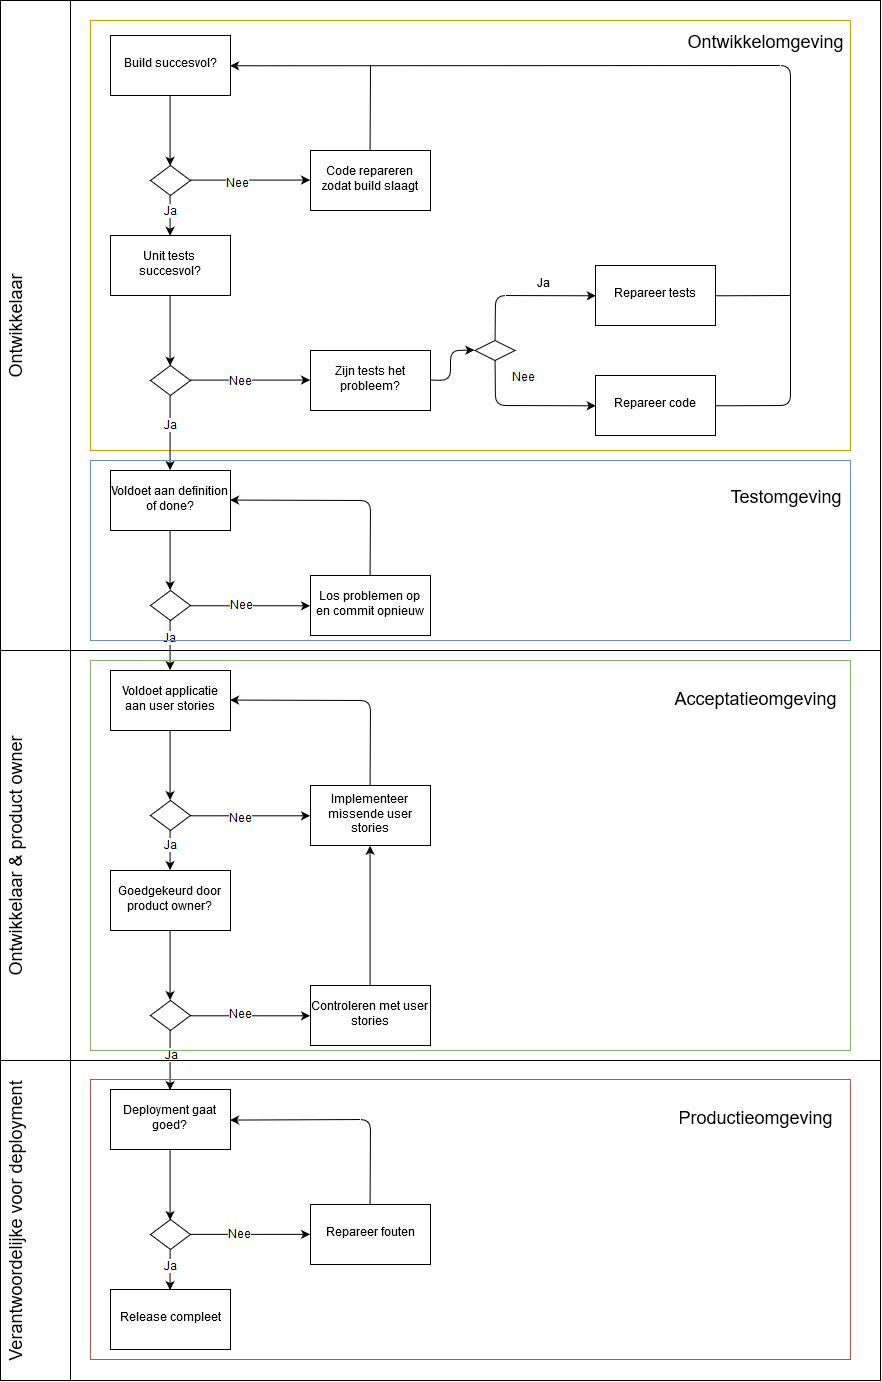
\includegraphics[width=0.6\textwidth]{images/ReleaseUML.png}
	\caption{Overzicht van het releaseproces}
\end{figure}

